\chapter{Sequences}
\label{ch:sequences}

%\begin{quote}
%  \emph{``Sequences are fundamental to the study of infinite series and many
%  applications of mathematics.''}
%
%\hfill\cite[p.~532]{thomas}
%\end{quote}
A \textbf{sequence}\index{sequence} is an ordered list of numbers. They are mostly important because of their application to \textbf{series},
detailed in Chapter~\ref{ch:series}.
\section{Representing a Sequence}
\begin{defn}
  A \textbf{sequence} is a list of numbers
  \[ a_1, a_2, a_3, \ldots, a_n, \ldots\]
  in a given order. This order is important: The sequence \(2, 4, 6, 8, \ldots\) is not the same as the sequence \(4, 2, 8, 6, \ldots\).
\end{defn}
When we write sequences like \(\{a_n\}\), we are talking about the entire
sequence. A sequence like this is described as ``starting at'' a certain \emph{index},
usually \(n=1\).
Most of the sequences we will be talking about will be infinite in length.

We can also write sequences using rules that describe their
terms, as follows:

\begin{ex}
\[ a_n = \frac{n!}{2n!+1} \]
  We can write out a few terms of the sequence
  \[
    \left\{
      \frac{1}{3},\frac{2}{5},\frac{6}{13},\frac{24}{49},\frac{120}{241},
    \ldots \right\}
  \]
  and then plot them %(shown in figure \ref{fig:firstsequence})
  to get a feel that the
  sequence is getting closer and closer to a certain number: \[ \frac{1}{2}.\] We would
  thus describe this sequence as \emph{converging to} the number \( \frac{1}{2} \)
% BROKEN FIGURE
%  \begin{figure}[h]
%    \begin{center}
%      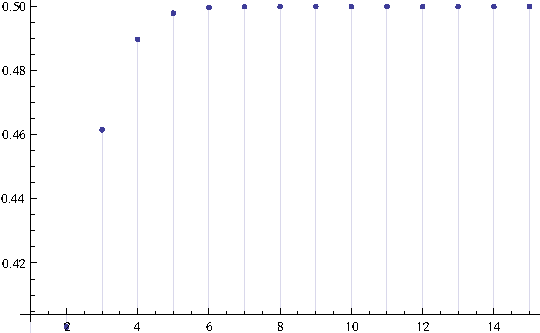
\includegraphics{graphs/nf2nfp1.pdf}
%    \end{center}
%    \label{fig:firstsequence}
%    \caption{A plot of \( a_n = \frac{n!}{2n!+1} \)}
%  \end{figure}
\end{ex}
\begin{defn}\index{converging sequence}
  The sequence \(\{ a_n \}\) \textbf{converges} to the number \(L\) if for every
  positive number \(\varepsilon\) there corresponds an integer \(N\) such that
  for all \(n\)
  \[ n > N \to |a_n - L| < \varepsilon \]
  If \(\{a_n\}\) converges to \(L\), we write \(\lim_{n \to \infty} a_n = L\),
  and call \(L\) the \emph{limit} of the sequence.
\end{defn}
  To really understand this, try thinking of it this way: pick a number $\varepsilon$. It can be very large
  \[ \varepsilon=1000\]
  or really small
  \[ \varepsilon=0.0001\]
  but no matter which one we pick, we can find an index $N$ on the sequence such that for every index past it, we
  are always within $\varepsilon$ of the limit $L$ for the sequence.
  Note that we don't have to know what this number $L$ is, nor what $\varepsilon$ is for that matter, just that
  these numbers exist to state that a sequence is \emph{converging}.
\begin{ex}
  Let us examine the following imaginary sequence:
  \begin{figure}[H]
    \begin{center}
      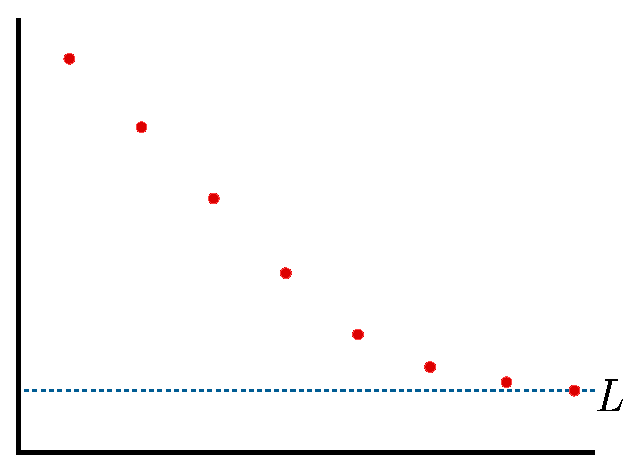
\includegraphics[scale=0.5]{continuous/sequence/conv1}
    \end{center}
    \label{fig:conv1}
  \end{figure}
  Note that for a large $\varepsilon$, our corresponding $N$ occurs very early in the sequence:
  \begin{figure}[H]
    \begin{center}
      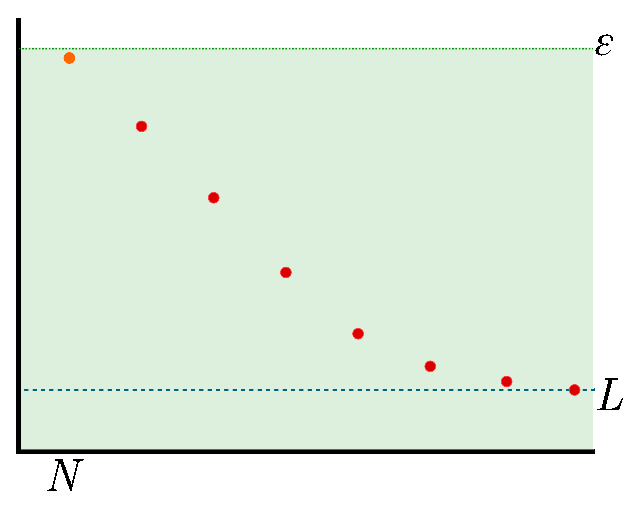
\includegraphics[scale=0.5]{continuous/sequence/conv2}
    \end{center}
    \label{fig:conv2}
  \end{figure}
  However, if we shrink our $\varepsilon$, the number $N$ needed such that every element in the sequence after it
  is within $\varepsilon$ of $L$ gets larger. The real key, however, is that it \emph{always exists}.
  \begin{figure}[H]
    \begin{center}
      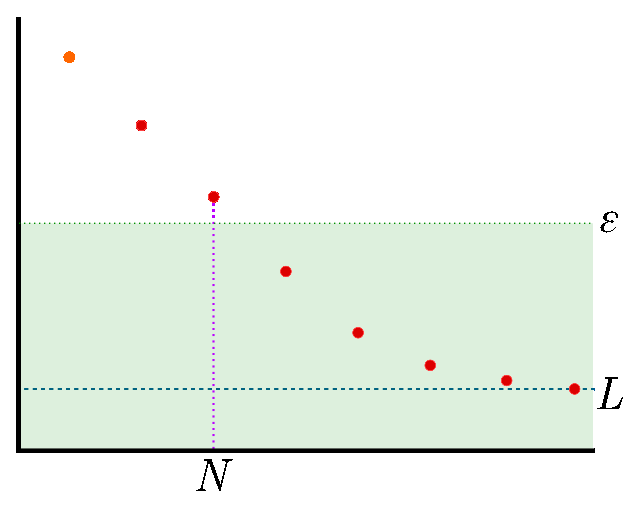
\includegraphics[scale=0.5]{continuous/sequence/conv3}
    \end{center}
    \label{fig:conv3}
  \end{figure}
\end{ex}
\begin{defn}\index{diverging sequence}
  The sequence \(\{ a_n \}\) \textbf{diverges} if the sequence does not converge
  to any number \(L\).

  That is, this number $L$ does not exist.
\end{defn}

\subsection{Bounded Sequences}
\begin{defn}\index{lower bound}
  If there exists a number $m$ such that $m \leq a_n$ for every $n$ we say the sequence is \textbf{bounded below}.
  The number $m$ is called a \textbf{lower bound} for the sequence.
  \begin{figure}[h]
    \begin{center}
      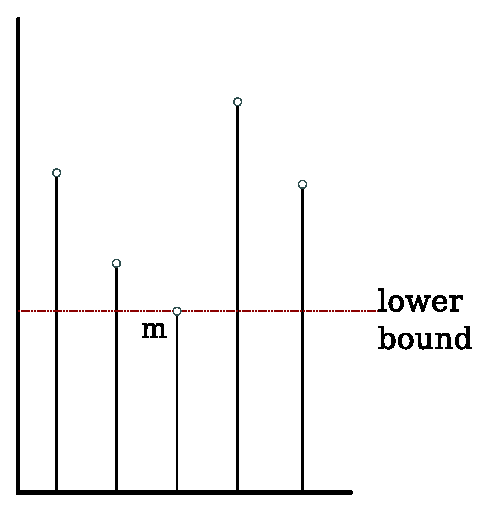
\includegraphics[scale=0.5]{continuous/sequence/lwrbnd}
    \end{center}
  \end{figure}
\end{defn}
\begin{defn}\index{upper bound}
  If there exists a number $M$ such that $a_n \leq M$ for every $n$ we say that the sequence is \textbf{bounded above}.
  The number $M$ is called an \textbf{upper bound} for the sequence.
  \begin{figure}[h]
    \begin{center}
      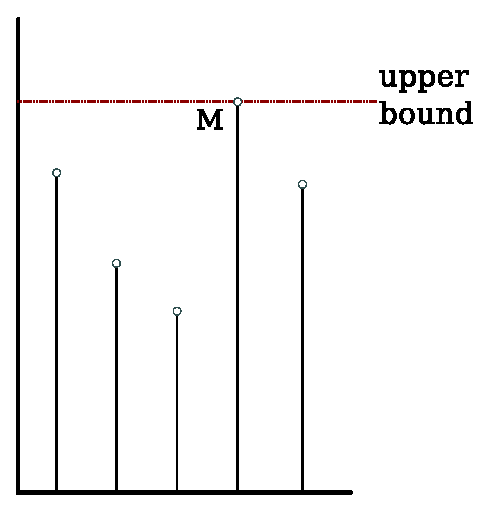
\includegraphics[scale=0.5]{continuous/sequence/uprbnd}
    \end{center}
  \end{figure}
\end{defn}
\begin{defn}\index{bounded}
  If the sequence is both bounded below and bounded above we call the sequence \textbf{bounded}.
\end{defn}
\subsection{Nondecreasing and Nonincreasing Sequences}\label{nondecreasing}
\begin{defn}\index{nondecreasing}
  Given a sequence \(\{a_n\}\), we call the sequence \textbf{nondecreasing} if
  \[\forall n (a_n \geq a_{n-1}).\]
  This means that across the entire sequence, a given element in the sequence is either greater than or equal to the preceding element.
  A nondecreasing sequence is different from a strictly \emph{increasing} sequence in that it allows for two elements to be equal.
  \begin{figure}[H]
    \begin{center}
      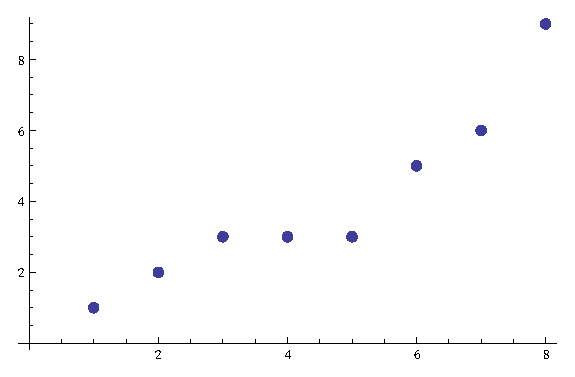
\includegraphics[scale=0.5]{continuous/sequence/nondecreasing}
    \end{center}
    \caption{This sequence is not \emph{increasing} everywhere, although it is \emph{nondecreasing}.}
  \end{figure}
\end{defn}
\begin{defn}
  Given a sequence \(\{a_n\}\), we call the sequence \textbf{nonincreasing} if
  \[\forall n (a_n \leq a_{n-1}).\]
\end{defn}
\begin{defn}
  If \(\{a_n\}\) is either nondecreasing or nonincreasing we call it \textbf{monotonic}.
  \begin{figure}[H]
    \begin{center}
      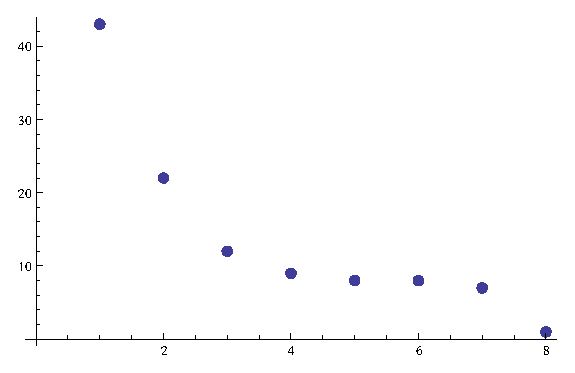
\includegraphics[scale=0.5]{continuous/sequence/nonincreasing}
    \end{center}
    \caption{An example of a nonincreasing sequence.}
  \end{figure}
\end{defn}

\begin{ex}\label{ex:bigsequence}
  \[ a_n=\frac{n+1}{2n-1} \]
    Let's take a more detailed look at an example of a sequence.

    To get a feel for the behavior of the sequence, let's find a few of its
    values:
    \[ \frac{n+2}{2n-1} =
      \left\{3,\frac{4}{3},1,\frac{6}{7},\frac{7}{9},\frac{8}{11}, \cdots \right\} \]


    We could take the derivative of the similar function
    \[ f(x)=\frac{x+2}{2x-1} \]
    to try to figure out what is happening. Since we can assume \(n \geq 1\) for
    our sequence, for \(x \geq 1\) the derivative of \(f(x)\) should also be
    somewhat representative of \(a_n\).
    \begin{align*}
      f'(x)&= \frac{(2 x-1) \left(\frac{\ud}{\ud x}(x+2)\right)-(x+2)
      \left(\frac{\ud}{\ud x}(2 x-1)\right)}{(2 x-1)^2}
      \\
      &=\frac{2 x-2 (x+2)-1}{(2 x-1)^2} \\
      &=-\frac{5}{1-4 x+4 x^2}
    \end{align*}
    \begin{table}[h]
      \centering
      \boxed{
        \begin{tabular}{>\(r<\)|>\(c<\)|>\(c<\)|>\(c<\)}
          x & 0 & 0.5 & 1 \\ \hline
          f'(x) & - & \text{undefined} & -
        \end{tabular}
      }
      \caption{A sign diagram for \(f'(x)\).}
      \label{tab:n51m2xs}
    \end{table}
    \begin{figure}[h]
      \begin{center}
        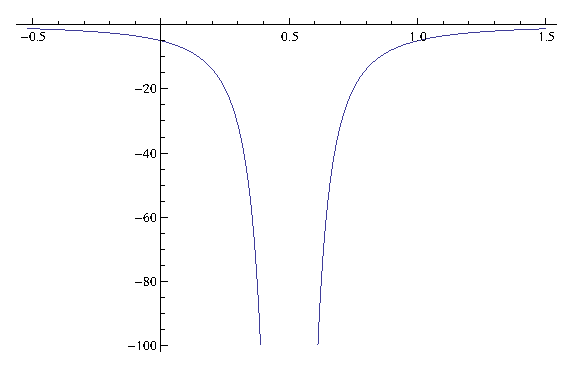
\includegraphics{graphs/n51m2xs}
      \end{center}
      \caption{A plot of \(f'(x)\).}
      \label{fig:n51m2xs}
    \end{figure}
    Based on Table \ref{tab:n51m2xs}, we can conclude that the sequence is
    nonincreasing. We can therefore describe this sequence as \emph{monotonic}.

    Furthermore, note the end-behavior of this derivative:
    \[ \lim_{x \to \infty} f'(x) = 0 \]
    This implies that, eventually, the rate of change evens off to an indefinitely small number.
    Presumably, this would mean that \(f(x)\) has a horizontal asymptote.
    Based on this information, it seems reasonable to conclude that the sequence \(a_n\) is converging upon a number.
    We do not, however, know to what number it converges.

    To find that, we will need to take the following limit:
    \[ \lim_{n\to\infty} a_n \]
    How do we evaluate limits for sequences? As it turns out, we usually treat
    them exactly the same as limits of functions, which are described in \chref{ch:limits}.
    \begin{theorem}\label{th:inftyanlimit}\index{limits of sequences}
      Suppose that \(f(x)\) is a function defined for all \( x \geq n_0\) and
      that \( \{a_n\} \) is a sequence of real numbers such that \(a_n = f(n)\)
      for \(n \geq n_0\). Then
      \[ \lim_{x \to \infty} f(x) = L \to \lim_{n \to \infty} a_n = L\text{.} \]
      \begin{proof}
        Suppose that \( \lim_{x \to \infty} f(x) = L \). Then for each positive
        number \( \varepsilon \) there is a number \( M \) such that for all
        \(x\),
        \[ x > M \implies \big| f(x) - L \big| < \varepsilon. \]
        Let \(N\) be an integer greater than \(M\) and greater than or equal to
        \(n_0\). Then
        \[ n > N \implies a_n = f(n),\]
        and
        \[\big|a_n -L \big| = \big|f(n) - L\big| < \varepsilon. \qedhere\]
        \cite[p. 537]{thomas}%Thomas' Calculus, p. 537
      \end{proof}
    \end{theorem}
    \thref{th:inftyanlimit} allows us to use \emph{l'Hospital's Rule} to find the limits of some
    sequences. We can state that
    \[\lim_{n\to\infty} a_n =\lim_{n\to\infty}f(x)\]
    assuming
    \[f(x)=\frac{n+1}{2n-1}\text{.}\]
    And thus evaluate the following limit:
    \begin{align*}
      \lim_{n\to\infty} \frac{n+1}{2n-1}
      &\=H \lim_{n\to\infty} \dfrac{\frac{\ud}{\ud x}(n+1)}{\frac{\ud}{\ud x}2n-1} \\
      &\=H \lim_{n\to\infty} \frac{1}{2} \\
      &= \frac{1}{2}
    \end{align*}
    This shows us that the sequence $a_n$ also converges to \(\frac{1}{2}\).
    \begin{figure}[H]
      \begin{center}
        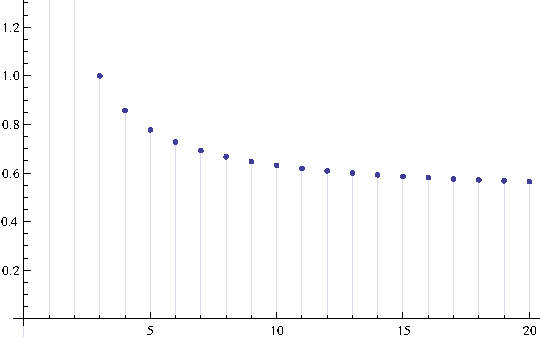
\includegraphics{graphs/np22nm1.pdf}
      \end{center}
      \caption{A graph of the sequence $ a_n=\frac{n+1}{2n-1} $.}
    \end{figure}
\end{ex}
\begin{ex}
  Demonstrate that $\{n!\}$ is nondecreasing.
  \begin{sol}
    First let us look at the definition for a factorial.
    \begin{equation}\label{eq:factorial}\index{factorial}
      n! =
      \begin{cases}
        1 & \text{if } n = 0, \\
        n(n-1)! & \text{if } n > 0
      \end{cases}
    \end{equation}
    \begin{proof}
      Remember our definition for a nondecreasing sequence from \ref{nondecreasing}:
      \[\forall n (a_n \geq a_{n-1})\text{.}\]
      Let us assume that this holds true for our sequence $\{n!\}$ when $n>1$.
      \begin{align*}
        n!&\geq(n-1)!& n&>1 \\
        \intertext{Divide each side by $(n-1)!$}
        \frac{n!}{(n-1)!}&\geq \frac{(n-1)!}{(n-1)!} &n&>1 \\
        \frac{n!}{(n-1)!}&\geq 1 &n&>1 \\
        \intertext{Now, remembering our definition for the factorial,}
        \frac{n(n-1)!}{(n-1)!}&\geq 1 &n&>1 \\
        n&\geq1 &n&>1\qedhere
      \end{align*}
    \end{proof}
    % \begin{proof}
    %   \begin{align*}
    %     \underbrace{n!}_{n(n-1)} > (n-1)!
    %     n(n-1)! &> (n-1)! \\
    %     n(n-1)! - (n-1)! &> 0 \\
    %     (n-1)! [n-1] &> 0 \qedhere
    %   \end{align*}
    % \end{proof}
  \end{sol}
\end{ex}
\begin{ex}
  Show that the sequence \[ \{a_n\} = \left\{ \frac{n+2}{2n-1} \right\}^{\infty}_{n=1} \] is nonincreasing.
  \begin{sol}
    This example is very similar to Example \ref{ex:bigsequence}, with only a
    change of constant in the numerator. We will demonstrate this sequence's
    behavior using a different method than before, however.

    Another way we can demonstrate that a sequence is decreasing is by using
    the definition of a \emph{decreasing sequence}: \(\forall n ( a_n <
    a_{n-1})\). We simply substitute in \(n\) and \(n-1\) on the
    respective sides of the inequality.
    \begin{proof}
      \begin{align*}
        \forall n (a_n &< a_{n-1}) &n&>1 \\
        \frac{n+2}{2n-1} &< \frac{(n-1)+2}{2(n-1)-1} &n&>1 \\
        \frac{n+2}{2n-1} &< \frac{n+1}{2n-3} &n&>1 \\
        \left(\frac{2n-3}{2n-3}\right) \left( \frac{n+2}{2n-1} \right)
        &< \left(\frac{n+1}{2n-3}\right) \left(\frac{2n-1}{2n-1}\right)
        &n&>1\\
        \frac{2n^2-3n+4n-6}{4n^2-6n-2n+3} &< \frac{2n^2+2n-n-1}{4n^2-6n-2n-3} &n&>1\\
        \frac{2n^2+n-6}{4n^2-8n+3}&<\frac{2n^2+n-1}{4n^2-8n-4} &n&>1 \\
        2n^2+n-6 &< 2n^2+n-1 &n&>1 \\
        -6 &< -1 &n&>1 \qedhere
      \end{align*}
    \end{proof}
  \end{sol}
\end{ex}
% \begin{ex}
%   Is
%   \[ \left\{\frac{n}{n+1} \right\} \]
%   monotonic?
%   \begin{sol}
%       \begin{align*}
%         \lim_{n\to\infty} \frac{n}{n+1}=1
%       \end{align*}
%       \begin{align*}
%         f(x)&=\frac{x}{x+1} \\
%         f'(x)&=\frac{(x+1)1-x(1)}{(x+1)^2} \\
%         f'(x)&=\frac{1}{(x+1)^2}
%       \end{align*}
%   \end{sol}
% \end{ex}
\begin{ex}
  Show that
  \[ \left\{ \frac{n}{n+1} \right\} \]
  is monotonic increasing.
  \begin{sol}
    \begin{proof}
      \[ \forall n > 1 \left(  a_n > a_{n-1}  \right) \]
      \begin{align*}
        a_n &> a_{n-1}\\
        \frac{n}{n+1} &> \frac{n-1}{n-1+1} \\
        \frac{n}{n} \frac{n}{n+1} &> \frac{n-1}{n}\frac{n+1}{n+1} \\
        n^2 &> (n-1)(n+1)\\
        n^2 &> n^2-1 \\
        0 &> -1 \qedhere
      \end{align*}
    \end{proof}
  \end{sol}
\end{ex}
\begin{ex}
  Does
  \[ a_n = \frac{n+1}{2^n} \]
  converge or diverge?
  \begin{sol}
    Remembering that we can rewrite \(2^n\) as
          \( e^{n \cdot \ln{2}} \)
    \begin{align*}
      \lim_{n \to \infty} \frac{n+1}{2^n}
      &= \lim_{n \to \infty} \frac{n+1}{e^{n\cdot \ln{2}}} \\
      &\=H \lim_{n \to \infty} \frac{1}{\ln2 \cdot e^{n\ln2}}\\
      &= \lim_{n \to \infty} \frac{1}{\ln2 \cdot 2^n}
      \intertext{Using the constant multiple rule for limits of sequences, we
      can pull out the \( \ln 2 \). }
      &= \frac{1}{\ln 2}\cdot \left(\lim_{n \to \infty}
      \frac{1}{2^n}\right)
    \end{align*}
    \(\{\frac{1}{2^n}\}\) is converging very quickly toward 0,
    so \(a_n\) as well must converge to \(0\).
    \begin{figure}[h]
      \begin{center}
        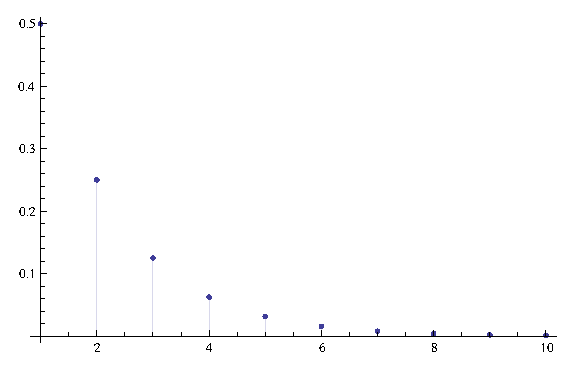
\includegraphics{graphs/oneovertwoton}
      \end{center}
      \caption{A plot of \(\{\frac{1}{2^n}\}\).}
      \label{fig:oneovertwoton}
    \end{figure}
  \end{sol}
\end{ex}
\begin{ex}
  Does
  \[ \left\{ \frac{1}{n!} \right\} \]
  converge or diverge?
  \begin{sol}
      \begin{align*}
        \lim_{n \to \infty} \frac{1}{n!} = 0
      \end{align*}
  \end{sol}
  Alternatively, we could demonstrate that the sequence is bounded and monotonic.
\end{ex}
\begin{ex}
  Does
  \[ a_n = \frac{2^n}{n!} \]
  converge or diverge?
  \begin{sol}
    We can show this, intuitively, as follows:
    \begin{align*}
      a_n = \left\{
        \frac{2\times2\times2\times2\times2\times\ldots}{1+2+3+4+5+6+\ldots} \right\}
    \end{align*}
    But the actual proof requires the \emph{sandwich theorem for
    sequences}\cite[p.~536]{thomas}:
    \begin{theorem}[The Sandwich Theorem for Sequences]\index{The Sandwich
      Theorem for Sequences}\label{th:sandwichsequence}
      Let $\{a_n\}$, $\{b_n\}$, and $\{c_n\}$ be sequences of real numbers. If
      $a_n \leq b_n \leq c_n $ holds for all $n$ beyond some index $N$, and if
      $\lim_{n\to\infty} a_n = \lim_{n\to\infty} c_n = L$, then
      $\lim_{n\to\infty} b_n = L$ also.
    \end{theorem}
      A proof of this theorem is found in \ref{proof:sandwichsequence}.
      By Theorem \ref{th:sandwichsequence}, \[\lim_{n \to \infty} a_n =
      \lim_{n\to\infty}\frac{2^n}{n!}=0.\]
  \end{sol}
\end{ex}
\begin{ex}
  \[ a_n = \frac{(-1)^n}{n!} \]
  \begin{sol}
    Consider
    \begin{align*}
      b_n = \left| \frac{(-1)^n}{n!} \right| = \frac{1}{n!} = 0
    \end{align*}
    Intuitively, we can also state that $a_n$ should converge.
    Using Theorem \ref{th:sandwichsequence}, we can determine that this sequence converges.
    % Review \emph{bounded and monotonic} for sequences, txtbg pg 536.
    % That's in Thomas' calculus. -[Nathan]
  \end{sol}
\end{ex}
\begin{ex}
  \[ a_n = \frac{1}{n-0.\bar{9}} \]
  \begin{sol}
    A sequence can be unbounded, and still converge.

    $0.\bar{9}$ is very close to $1$, close enough that we can treat it as $1$ as $n\to\infty$.
    Doing so, it becomes clear that this sequence converges, as $\frac{1}{n-1}$ converges.
    Consider, however, the very first term, where $n=1$.
    This term is \emph{gigantic}, essentially \(\infty\).
    The sequence is not bounded, yet it still manages to converge.
    This sequence converges to \(0\).
  \end{sol}
\end{ex}
\begin{ex}
  Does the following sequence converge?
  \[ a_n = \left( \frac{n+8}{9n} \right) \left( 1-\frac{8}{n} \right) \]
  Find the limit if the sequence is convergent.
  \begin{sol}
    Remembering that a limit of products is a product of limits,
    \begin{align*}
      \lim_{n \to \infty} \left( \frac{n+8}{9n} \right) \left( 1-\frac{8}{n} \right)
      &= \lim_{n \to \infty} \left( \frac{n+8}{9n} \right) \cdot
      \lim_{n \to \infty} \left( 1-\frac{8}{n} \right)\\
      &= \frac{1}{9}
    \end{align*}
    The sequence converges to \(\frac{1}{9} \).
  \end{sol}
\end{ex}
\begin{ex}
  Show that the sequence \[a_n = \frac{2}{n^2} \] is monotonic and bounded.
  \begin{sol}
    Treat the sequence as a function $f(x)$ and take the derivative.
    \[ f(x) = \frac{2}{x^2} \]
    \[ f'(x) = -4 x^{-3} \]
    $f'(x)$ is negative on the interval $[1, \infty)$, so $f(x)$ is decreasing
      on the interval $[1, \infty)$. Since the sequence goes from $1$ to
        $\infty$ and is always decreasing, its upper bound must be at $n=1$.
        $a_1=2$, the upper bound for the sequence. To find the lower bound, we
        take the limit as $n \to \infty$:
        \[ \lim_{n \to \infty} a_n = \lim_{n \to \infty} \frac{2}{n^2} = 0 \]
        Which shows us that $0$ is the lower bound of the sequence.

        Thus, we can conclude that the sequence is monotonic and bounded, and therefore converges.
  \end{sol}
\end{ex}
\begin{ex}
  Find a formula for the nth term of the sequence where \(a_n\) is calculated
  directly from \(n\).
  \[ \frac{1}{1}, \frac{4}{2}, \frac{7}{6}, \frac{10}{24}, \frac{13}{120} \cdots \]
  \begin{sol}
    We basically have to just take close guesses and see if we can make a sequence that follows this.

    Doing so, we will find that the answer is
    \[ a_n = \frac{3n-2}{n!}.\]
  \end{sol}
\end{ex}

% \begin{homework}
%     Wolfram Mathematica assingment and MyMathLab homework due Friday, March 23, 2012.
% \end{homework}
% \begin{homework}
%   Read Section 10.2
%
%   pg. 551 ALL 27-34, 35, 36, 37, 38, 41, 43, 49, 50, 51, 55, 56, 57, 58, 59, 61
% \end{homework}
%
